\documentclass[useAMS, usenatbib, a4paper]{mnras}
\usepackage[spanish,es-minimal,english]{babel}
\usepackage[utf8]{inputenc}
\usepackage{graphicx}
\usepackage{xcolor}
\usepackage{fixltx2e}
\usepackage{hyperref}
\usepackage{savesym}
\savesymbol{tablenum}
\usepackage{siunitx}
\restoresymbol{SIX}{tablenum}
\usepackage{newtxtext}
\usepackage[varg,varvw,smallerops]{newtxmath}
\usepackage{xfrac} % for the \sfrac macro
\usepackage{booktabs}
\usepackage{array}   % for \newcolumntype macro
\bibliographystyle{mnras}

% A better \ion command that works in more circumstances
\newcommand\ION[2]{#1\,\scalebox{0.9}[0.8]{\uppercase{#2}}}
\newcounter{ionstage}
\renewcommand{\ion}[2]{\setcounter{ionstage}{#2}% 
  \ensuremath{\mathrm{#1\,\scriptstyle\Roman{ionstage}}}}
\newcommand\hii{\ion{H}{2}}

% Stars in Orion, e.g., \th1C, \th2A
\def\th#1#2{\(\theta^{#1}\)\,Ori~#2}
% Wavenumbers
\newcommand\wn{\ensuremath{\tilde{\nu}}}

% Chemical formulae
\newcommand*\chem[1]{\ensuremath{\mathrm{#1}}}
% Atomic term symbols
\newcommand\Config[1]{\ensuremath{\mathrm{#1}}}
\newcommand\Term[3]{\ensuremath{\mathrm{#1\ ^{#2}#3}}}
\newcommand\Level[4]{\ensuremath{\mathrm{#1\ ^{#2}#3_{#4}}}}

% Emission lines
\newcommand\ha{\ensuremath{\text{H}\alpha}}
\newcommand\lya{\ensuremath{\text{Ly}\alpha}}
\newcommand\lyb{\ensuremath{\text{Ly}\beta}}
\newcommand\Raman{\ensuremath{_{\text{Raman}}}}
\newcommand\FUV{\ensuremath{_{\text{FUV}}}}


\title[Raman mapping of Orion PDRs]
{Raman mapping of photodissociation regions in Orion}

\author[Henney]{
  William J. Henney\thanks{w.henney@irya.unam.mx}\\
  \foreignlanguage{spanish}{Instituto de Radioastronomía y
    Astrofísica, Universidad Nacional Autónoma de México, Apartado
    Postal 3-72, 58090 Morelia, Michaoacán, Mexico}}

% These dates will be filled out by the publisher
\date{Accepted XXX. Received YYY; in original form ZZZ}

% Enter the current year, for the copyright statements etc.
\pubyear{2019}

\begin{document}
\label{firstpage}
\pagerange{\pageref{firstpage}--\pageref{lastpage}}
\maketitle
\begin{abstract}
  I show that the broad Raman-scattered wings of H\(\alpha\) can be used to
  map neutral gas illuminated by high-mass stars in star forming
  regions. The near wings
  (\(\Delta\lambda \approx \pm \SI{10}{\angstrom}\)) trace neutral hydrogen columns of
  about \SI{5e20}{cm^{-2}}, while the farther wings
  (\(|\Delta\lambda| > \SI{30}{\angstrom}\)) trace columns of about
  \SI{5e21}{cm^{-2}}. Absorption features in the pseudo-continuum at
  6633 and 6664~\AA{} correspond to neutral oxygen far-ultraviolet
  absorption lines at \SIlist{1027.43;1028.16}{\angstrom}.
\end{abstract}
\begin{keywords}
  Atomic physics -- Radiative transfer -- Photodissociation regions
\end{keywords}
%\facilities{VLT:Yepun (MUSE); OANSPM:2.1m (Mezcal); Keck (HIRES)}
%\object{M42}
\section{Introduction}
\label{sec:introduction}
Raman scattering is the inelastic analog of Rayleigh scattering by
atoms or molecules.  Both processes begin with a radiation-induced
transition of an electron to a virtual bound state (non-eigenstate).
In Rayleigh scattering, the electron returns to its original state,
resulting in the radiation being re-emitted with its original
frequency (elastic scattering).  In Raman scattering, on the other
hand, the electron undergoes a transition to a different excited
state, resulting in radiation being re-emitted at a much lower
frequency.  See Figure~\ref{fig:raman-cartoon} for an illustration of
the process.

\begin{figure}
  \centering
  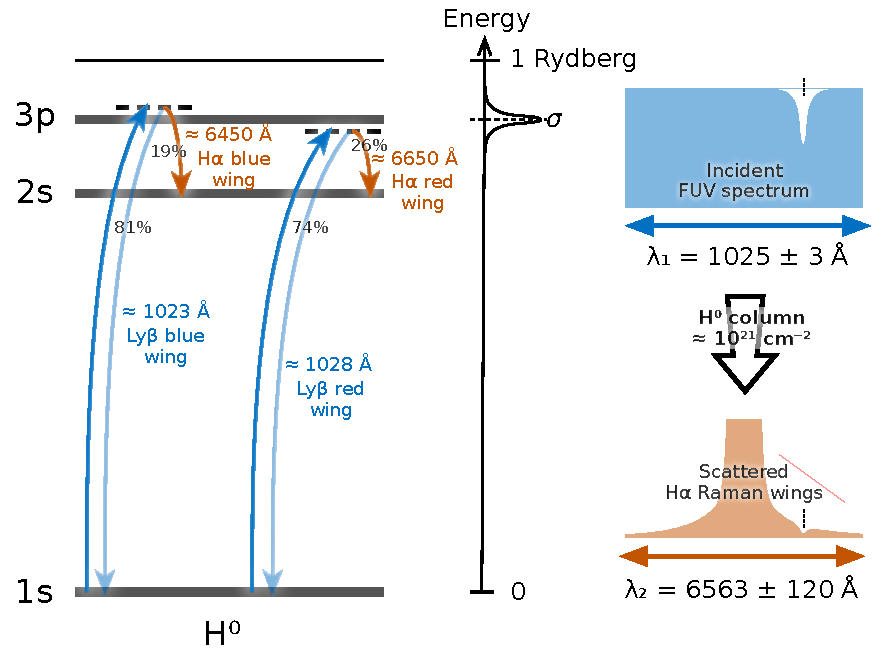
\includegraphics[width=\linewidth]{figs/raman-cartoon}
  \caption{Schematic illustration of Raman scattering of photons from
    the \lyb{} wings to the \ha{} wings.  The relevant energy levels
    of neutral hydrogen are shown at left.  Far ultraviolet photons
    that are shifted by about \(\Delta\lambda_1 = \pm 1\) to \SI{3}{\angstrom}
    from the \lyb{} rest wavelength can excite transitions from the
    ground \Config{1s} level to a virtual state adjacent to
    \Config{3p}.  Most such excitations decay back to \Config{1s}
    (Rayleigh scattering), but in about one-fifth of cases the decay
    is to \Config{2s} instead (Raman scattering).  The scattering
    cross section falls approximately as \(\Delta\lambda_1^{-2}\), which gives
    broad Lorentzian wings to the \ha{} line, as shown at right. A
    bandwidth of \(\Delta\lambda_1 = \pm \SI{3}{\angstrom}\) around \lyb{} is
    transformed to a bandwidth
    \(\Delta\lambda_2 \approx \pm \SI{120}{\angstrom}\) around \ha{}.  A narrow
    absorption line in the incident FUV spectrum (vertical thin dashed
    line) becomes a much broader notch in the scattered wings.}
  \label{fig:raman-cartoon}
\end{figure}

Here is another paragraph, which I have written in overleaf. Now I add another sentence to this paragraph.

\end{document}
